% PLOS Computational Biology draft.
% Skeleton follows the PLOS structure (Abstract, Author Summary, Introduction,
% Results, Discussion, Materials & Methods). Before submission, port into the
% official PLOS template (plos_latex_template.tex + plos2015.bst from
% journals.plos.org); this draft uses article + unsrtnat so co-authors can
% build it anywhere with a stock TeX distribution.
\documentclass[10pt,letterpaper]{article}
\usepackage[top=0.85in,left=1.2in,right=1.2in,bottom=1.0in]{geometry}
\usepackage{amsmath,amssymb}
\usepackage{graphicx}
\usepackage{booktabs}
\usepackage[numbers,sort&compress]{natbib}
\usepackage{tikz}
\usetikzlibrary{arrows.meta,positioning,fit,calc}
\usepackage[colorlinks=true,linkcolor=blue,citecolor=blue,urlcolor=blue]{hyperref}
\usepackage{xspace}
\newcommand{\Rt}{\ensuremath{R_t}\xspace}
\graphicspath{{figs/}}

\title{\vspace{-1.2em}\textbf{A neural epidemic forecaster that learns its own
generation interval}}

\author{%
Michael Ajao-Olarinoye$^{1,\ast}$ \and
[co-authors to be confirmed]$^{2}$\\[0.6em]
\small $^{1}$Centre for Computational Science and Mathematical Modelling,
Coventry University, Coventry, UK\\
\small $^{\ast}$Corresponding author: ajaoolarinoyemichael@gmail.com}
\date{Draft of 20 August 2026 --- for circulation to prospective co-authors}

\begin{document}
\maketitle

\begin{abstract}
Internal quantities of neural epidemic forecasters are often given
epidemiological names, but the correspondence is rarely tested. We equip a
graph neural forecaster with a decoder that implements the renewal equation of
infectious-disease epidemiology, with the generation-interval kernel treated
as a free parameter vector and learned jointly with the rest of the network,
and we test whether the learned quantities agree with their classical
counterparts. Trained on daily COVID-19 hospital admissions for the seven
English NHS regions, with no epidemiological supervision, the model recovers a
mean generation interval between 3.2 and 4.5 days at forecast horizons of 3,
7 and 14 days; 14 of 15 independently seeded models fall inside the 3--5 day
range reported from contact-tracing studies, and the seed-to-seed standard
deviation at the shortest horizon is 0.06 days. The reproduction number
implied by the decoder correlates with a Cori-type EpiEstim estimate at
$r=0.94$ in aggregate, and in every region separately at short horizons; we
show that comparable correlation is attainable by model-free growth
statistics and interpret it accordingly. Freezing
the kernel, either to a flat distribution or to the published literature
value, degrades validation accuracy relative to the learned kernel. On the
held-out test split the renewal decoder attains equal or lower error than an
unconstrained decoder and reduces seed variance roughly tenfold at short
horizons, although no difference reaches significance with five seeds. On the
validation split used for model selection, in contrast, none of nine renewal
configurations outperformed the unconstrained decoder, and the exact iterated
formulation was worse than an approximate one. Mechanistic fidelity and point
accuracy therefore behave as separate objectives in this setting, and the
benefit of structural assumptions depends strongly on forecast horizon.
\end{abstract}

\subsection*{Author summary}
Machine-learning models are increasingly used to forecast epidemics, and their
internal workings are often described in epidemiological language: attention
weights become ``transmission pathways'', latent variables become
``transmissibility''. Such descriptions are seldom checked. We built a
forecaster whose final stage is the renewal equation, the standard model of
epidemic transmission, and left one of its key ingredients, the generation
interval between successive infections, for the network to estimate from data.
Trained only on daily hospital admissions for the English NHS regions, the
model arrived at a generation interval of roughly three to four and a half
days, in agreement with published estimates for COVID-19 obtained from
contact tracing. The reproduction number it computes internally closely
matches the EpiEstim method used by public-health agencies, although the model
was never shown either quantity. Building in the mechanism did not make point
forecasts more accurate, and at very short horizons the model learned to
bypass the mechanism altogether. We conclude that a forecaster can be
mechanistically faithful without being more accurate, and that the two
properties should be evaluated separately.

\section{Introduction}

Epidemic forecasts inform decisions: staffing a hospital, timing an
intervention, issuing a public warning. The people making those decisions need
to know not only what a model predicts but why, because a forecast that rises
through increasing transmissibility calls for a different response from one
that rises because a reporting backlog cleared. Public-health agencies already
maintain a quantity that answers this question, the instantaneous reproduction
number, and interpret it daily. Neural forecasters usually expose nothing
comparable. Their internal states are described in epidemiological language,
attention weights as ``transmission pathways'' or latent variables as
``transmissibility'', but those descriptions are rarely tested, and a quantity
merely named after a mechanism cannot be audited against an agency's own
estimate of it. Two consequences follow: an accurate neural forecast remains
hard to reconcile with the surveillance apparatus around it, and claims about
learned dynamics reach policy-facing tools without being checked.

We take the narrowest version of this problem that admits a decisive test. If
a forecaster is built so that its final stage is the standard transmission
model of epidemiology, the quantities inside that stage acquire definite
classical counterparts, and whether the model ``learns transmission dynamics''
becomes a measurement rather than an interpretation.

The renewal equation relates incidence $I(t)$ to the instantaneous
reproduction number \Rt through a convolution with the generation-interval
distribution $w_\tau$,
\begin{equation}
  I(t) \;=\; R_t \sum_{\tau \geq 1} w_\tau\, I(t-\tau).
  \label{eq:renewal}
\end{equation}
It underlies the estimators of Fraser~\cite{fraser2007estimating} and Cori et
al.~\cite{cori2013new}, the EpiEstim and EpiNow2
software~\cite{cori2013new,abbott2020estimating} used by public-health
agencies, and semi-mechanistic Bayesian models of intervention
effects~\cite{flaxman2020estimating}. In all of these, $w_\tau$ is fixed in
advance: a generation interval measured from contact-tracing data, for example
a mean of 5.2 days for ancestral SARS-CoV-2~\cite{ferretti2020quantifying}, is
supplied to the estimator. Misspecification of $w_\tau$ is a recognised
source of bias in \Rt estimation~\cite{gostic2020practical}. The generation
interval is not an incidental input: Wallinga and
Lipsitch~\cite{wallinga2007generation} showed that the reproduction number and
the epidemic growth rate are related by a transform whose form is fixed
entirely by the shape of $w_\tau$, so which generation interval one assumes
determines which reproduction number one infers from the same data.

Neural forecasters sit at the other extreme. Spatiotemporal graph models such
as Cola-GNN~\cite{dengColaGNNCrosslocationAttention2020a},
EpiGNN~\cite{xie2022epignn} and DCRNN~\cite{li2017diffusion} learn flexible
representations without mechanistic constraints, and their attention maps are
frequently given epidemiological readings; related delay-aware attention
mechanisms exist outside epidemiology~\cite{jiang2023pdformer,press2022train,
shaw2018self}. Hybrid models incorporate compartmental structure as a loss
term or driving signal~\cite{gao2021stan,cao2022mepognn}. The mechanistic
quantities inside such models are, however, rarely compared against the
classical estimators they are named after. In companion work (in preparation)
we found that an attention module described in mechanistic terms in an earlier
version of this model was in fact inert, while the surrounding model forecast
adequately; that experience motivates the present study.

Here we attach a renewal decoder to a fixed neural backbone. The network
outputs $\log R$ per region and per step, and incidence is reconstructed
through Eq.~\eqref{eq:renewal} with a learned kernel
$\alpha_\tau=\mathrm{softmax}(\theta)_\tau$ and a learned spatial coupling.
The backbone, data, splits and training procedure are identical to those of
the unconstrained decoder, so comparisons isolate the decoder. Several of these ingredients exist separately. Renewal
recursions are already implemented in automatic-differentiation frameworks:
PyRenew, maintained by the US Centers for Disease Control and Prevention,
expresses exactly Eq.~\eqref{eq:renewal} in NumPyro/JAX, though it treats
$w_\tau$ as a fixed user-supplied input~\cite{cdc2024pyrenew}. Differentiability
alone is therefore not the contribution. Mechanistic epidemic simulators have
been made differentiable and calibrated by gradient descent, learning a
time-varying reproduction number but not an infectiousness
kernel~\cite{chopra2023gradabm}. Generation intervals have been estimated from
surveillance counts jointly with a dynamic reproduction number, by
expectation--maximisation over a parametric Weibull family inside a Hawkes
model~\cite{chiang2022hawkes}, and self-exciting triggering kernels have been
learned end-to-end inside neural encoders as a replacement for
attention~\cite{isik2023hawkes,turkmen2021deep}, though on clinical event
sequences rather than epidemic incidence. A concurrent preprint makes classical
\Rt inference differentiable but keeps $w_\tau$ fixed and names joint inference
of the kernel as future work~\cite{cirl2026conditional}.

What we have not found is the specific combination studied here: a
\emph{nonparametric} generation-interval kernel learned by gradient descent
\emph{inside a spatially coupled neural forecaster}, with the recovered kernel
and the reproduction number it implies both checked against classical
epidemiological estimates. Each qualifier is load-bearing, and we state the
claim at that resolution rather than more broadly.

The contributions are as follows. First, a renewal decoder for graph neural
forecasters in which the generation interval is a trained parameter
(Sec.~\ref{sec:methods}). Second, evidence that the learned kernel is
meaningful: it reproduces published COVID-19 generation intervals across
horizons and seeds (Sec.~\ref{sec:gi}), and forecasts deteriorate when it is
replaced by a flat or literature-fixed kernel (Sec.~\ref{sec:arms}). Third, a
comparison of the implied reproduction number with EpiEstim, in aggregate and
per region (Sec.~\ref{sec:rt}). Fourth, a complete account of the accuracy
results, including the search record in which no renewal configuration beat
the unconstrained decoder on the selection split (Sec.~\ref{sec:test},
\ref{sec:sweep}). Fifth, a description of how the value of structural
assumptions varies with forecast horizon, observed in four separate analyses
(Sec.~\ref{sec:threshold}).

\begin{figure}[ht]
\centering
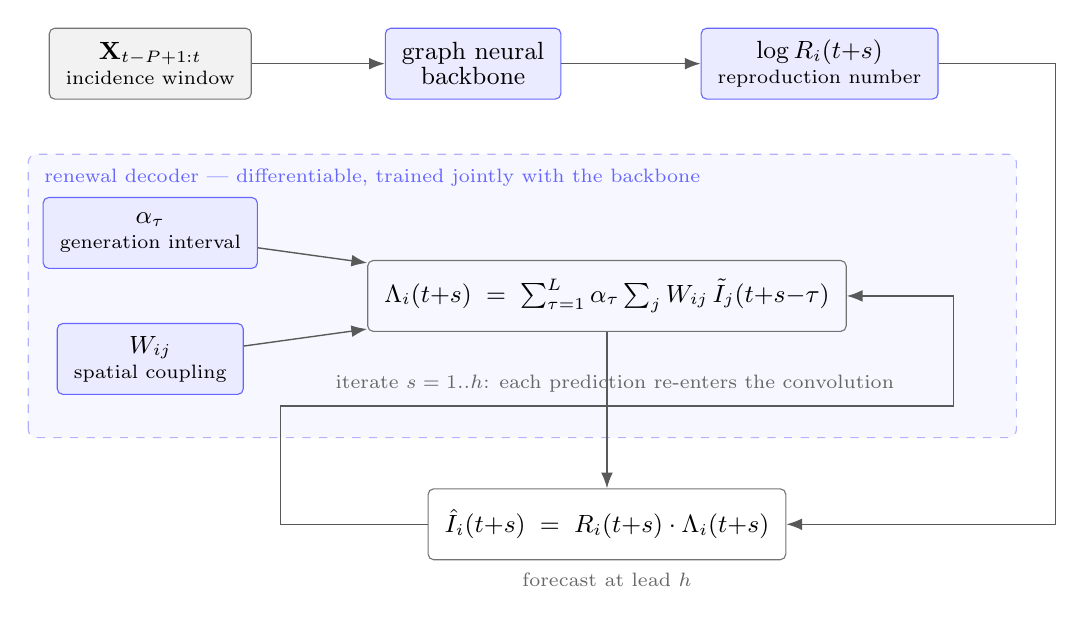
\begin{tikzpicture}[
  font=\small,
  box/.style={draw=black!55, rounded corners=2pt, minimum height=9mm,
              inner xsep=6pt, align=center},
  learn/.style={box, fill=blue!8, draw=blue!60},
  data/.style={box, fill=black!5},
  ar/.style={-{Latex[length=2mm]}, draw=black!65, line width=0.5pt},
  lbl/.style={font=\scriptsize, text=black!60}]

% panel behind the decoder stage
\fill[blue!3, rounded corners=3pt] (-2.15,-4.75) rectangle (10.4,-1.15);
\draw[blue!30, dashed, rounded corners=3pt] (-2.15,-4.75) rectangle (10.4,-1.15);
\node[lbl, text=blue!60, anchor=north west] at (-2.07,-1.22)
     {renewal decoder --- differentiable, trained jointly with the backbone};

% backbone row
\node[data]  (x)  at (-0.6,0) {$\mathbf{X}_{t-P+1:t}$\\[-2pt]\scriptsize incidence window};
\node[learn] (bb) at (3.5,0)  {graph neural\\[-2pt]backbone};
\node[learn] (R)  at (7.9,0)  {$\log R_i(t{+}s)$\\[-2pt]\scriptsize reproduction number};
\draw[ar] (x)  -- (bb);
\draw[ar] (bb) -- (R);

% decoder inputs
\node[learn] (al) at (-0.6,-2.15) {$\alpha_\tau$\\[-2pt]\scriptsize generation interval};
\node[learn] (W)  at (-0.6,-3.75) {$W_{ij}$\\[-2pt]\scriptsize spatial coupling};
\node[box]   (conv) at (5.2,-2.95)
     {$\Lambda_i(t{+}s)\;=\;\sum_{\tau=1}^{L}\alpha_\tau
       \sum_j W_{ij}\,\tilde I_j(t{+}s{-}\tau)$};
\draw[ar] (al) -- (conv);
\draw[ar] (W)  -- (conv);

% output below the panel
\node[box] (out) at (5.2,-5.85)
     {$\hat I_i(t{+}s)\;=\;R_i(t{+}s)\cdot\Lambda_i(t{+}s)$};
\draw[ar] (conv) -- (out);
% log R enters the product from the right, clear of the panel
\draw[ar] (R.east) -- (10.9,0) -- (10.9,-5.85) -- (out.east);

% feedback: prediction re-enters the convolution
\draw[ar] (out.west) -- (1.05,-5.85) -- (1.05,-4.35) -- (9.6,-4.35)
          -- (9.6,-2.95) -- (conv.east);
\node[lbl, anchor=south] at (5.3,-4.30)
     {iterate $s=1..h$: each prediction re-enters the convolution};
\node[lbl, anchor=north] at (5.2,-6.35) {forecast at lead $h$};
\end{tikzpicture}
\caption{The renewal decoder. A graph neural backbone outputs $\log R$ per
region and per forecast step; the decoder reconstructs incidence through the
renewal equation using a learned generation-interval kernel $\alpha_\tau$ and a
learned spatial coupling $W_{ij}$. Shaded blocks contain trained parameters.
The decoder is iterated: each predicted step re-enters the convolution, so
$\alpha_\tau$ indexes a delay from the forecast step. The three arms of the
study differ only in whether $\alpha_\tau$ is free (learned), frozen flat
(uniform), or frozen to a literature value (fixed).}
\label{fig:arch}
\end{figure}

\section{Results}

\subsection{Recovered generation intervals}
\label{sec:gi}

We trained the renewal model on daily COVID-19 hospital admissions for the
seven English NHS regions at forecast horizons $h\in\{3,7,14\}$ days, with
five random seeds per horizon. The loss is computed from case counts only.
Because the decoder is iterated, rolling Eq.~\eqref{eq:renewal} forward $h$
steps and feeding its own predictions back, kernel index $\tau$ measures a
delay from the forecast step and can be compared directly with a generation
interval.

\begin{table}[ht]
\centering
\caption{Mean delay of the learned kernel $\alpha_\tau$ ($\tau=1..7$ days) per
horizon, over five independently seeded models. Contact-tracing estimates of
the COVID-19 generation interval are approximately 3--5
days~\cite{ferretti2020quantifying}.}
\begin{tabular}{lcccc}
\hline
Horizon & Seeds & Mean delay (d) & Range (d) & In 3--5\,d range \\
\hline
$h=3$ & 5 & $3.23 \pm 0.06$ & [3.18, 3.33] & 5/5 \\
$h=7$ & 5 & $4.52 \pm 0.34$ & [4.19, 5.02] & 4/5 \\
$h=14$ & 5 & $3.62 \pm 0.37$ & [3.18, 4.05] & 5/5 \\
\hline
\end{tabular}

\label{tab:gi}
\end{table}

Mean recovered delays are $3.23\pm0.06$, $4.52\pm0.34$ and $3.62\pm0.37$ days
at $h=3,7,14$ respectively (Table~\ref{tab:gi}, Fig~\ref{fig:kernels}); 14
of the 15 models lie inside the published 3--5 day range. The comparison
benchmark deserves care. Ganyani et al.~\cite{ganyani2020estimating} estimate
the COVID-19 mean generation interval by Bayesian data augmentation from
symptom-onset clusters as 5.20 days (95\% CrI 3.78--6.78) in Singapore and
3.95 days (95\% CrI 3.01--4.91) in Tianjin; our recovered values sit inside the
Tianjin credible interval and at the lower edge of the Singapore one. Moreover,
intervals reconstructed by looking backward from observed cases are
systematically shorter than forward intervals during exponential
growth~\cite{park2021forward}, so contact-tracing benchmarks are themselves
sensitive to how they were collected. We therefore treat agreement with the
published range as consistency rather than as a point identification. At $h=3$ the
recovery is nearly identical across seeds. These figures establish a stable,
quantitative recovery of a plausible delay distribution from case counts
alone. They do not establish that the model has identified the biological
generation interval; Sec.~\ref{sec:discussion} describes a confound that is
visible in the kernel's shape.

\begin{figure}[ht]
\centering
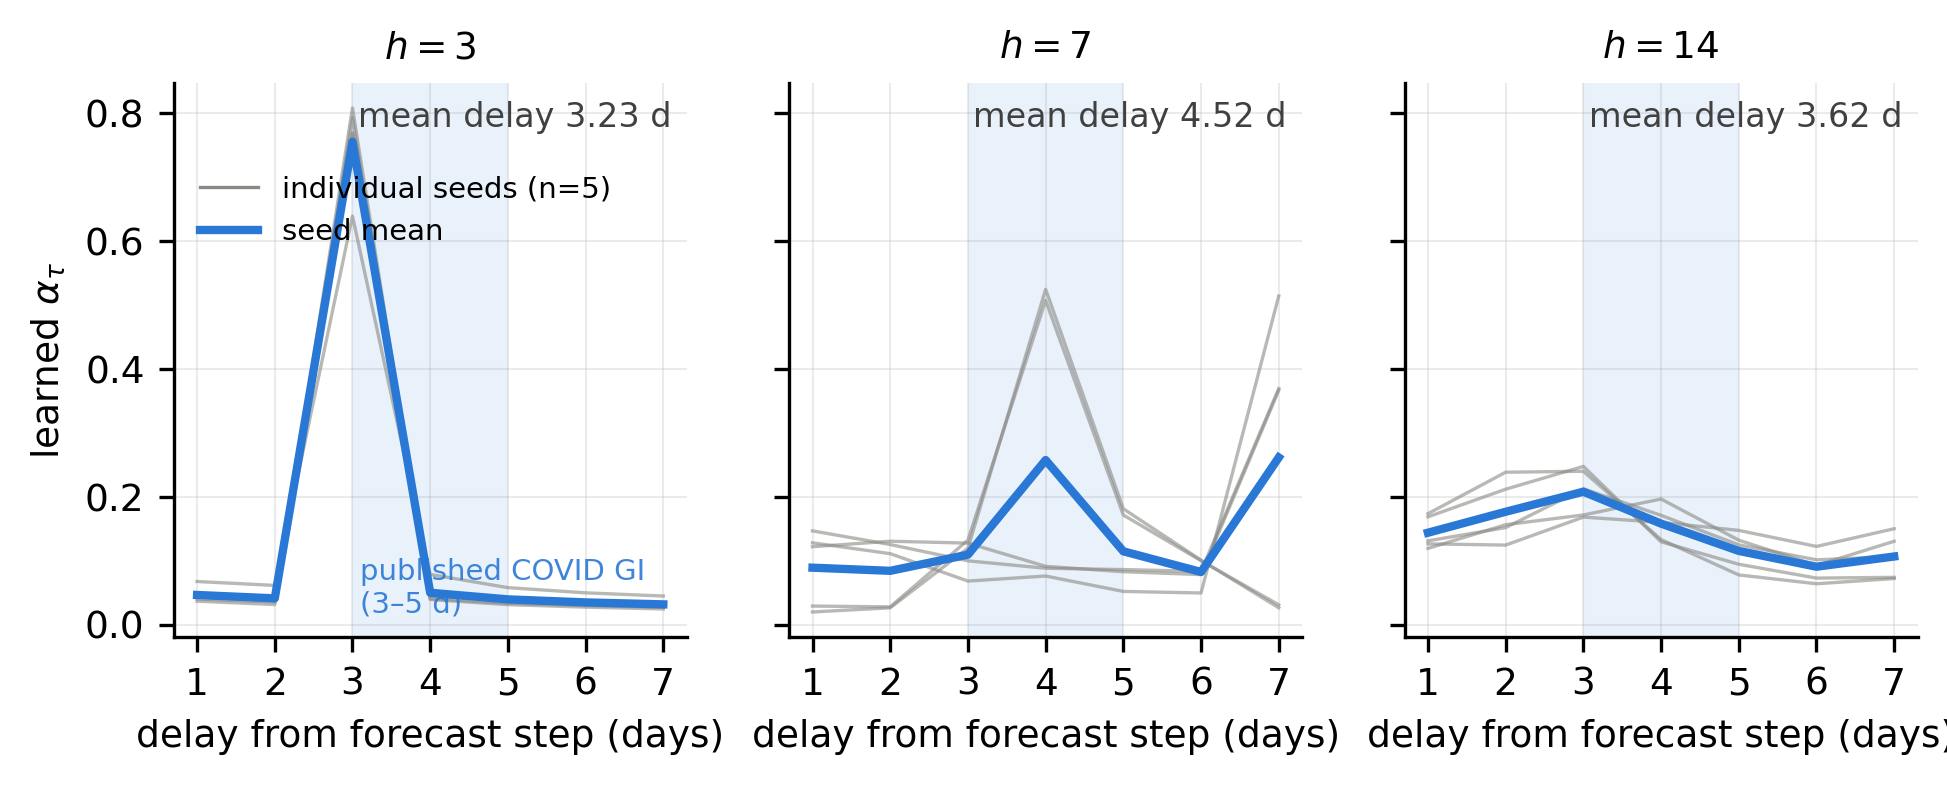
\includegraphics[width=\linewidth]{F2_gi_kernels}
\caption{Learned generation-interval kernels: per-seed kernels (grey, $n=5$)
and their mean (blue) at each horizon. The shaded band marks the published
3--5 day COVID-19 generation interval. The $h=3$ kernel concentrates at
$\tau=3$, which is also the delay at which the iterated decoder reaches the
last observed value (see Discussion).}
\label{fig:kernels}
\end{figure}

\subsection{Effect of freezing the kernel}
\label{sec:arms}

A recovered kernel could in principle have no influence on the forecasts. To
test this we compare three arms that share one backbone and differ only in
$\alpha_\tau$: \emph{learned} (free), \emph{uniform} (frozen flat), and
\emph{fixed} (frozen to the discretised literature gamma with mean 5.2 d, SD
1.72 d~\cite{ferretti2020quantifying}).

\begin{table}[ht]
\centering
\caption{Validation RMSE of the three kernel arms (NHS, mean $\pm$ SD over
five seeds; bold marks the lowest mean). The learned kernel has the lowest
mean at $h=3$ and $h=7$ and the lowest seed variance at all three horizons
except $h=14$.}
\begin{tabular}{lcccc}
\hline
Horizon & Direct decoder & Learned & Uniform & Fixed (lit.) \\
\hline
$h=3$ & $3.37 \pm 0.71$ & $\mathbf{3.00 \pm 0.17}$ & $3.77 \pm 1.46$ & $3.83 \pm 1.17$ \\
$h=7$ & $\mathbf{8.56 \pm 0.85}$ & $9.01 \pm 0.84$ & $9.70 \pm 1.16$ & $9.99 \pm 1.54$ \\
$h=14$ & $\mathbf{17.24 \pm 2.44}$ & $18.88 \pm 2.25$ & $19.11 \pm 2.04$ & $18.38 \pm 1.63$ \\
\hline
\end{tabular}

\label{tab:arms-val}
\end{table}

The learned arm attains lower validation error than the uniform kernel at all
three horizons (mean difference $-9.6\%$) and lower error than the literature
kernel at two of three (mean $-9.6\%$), and its seed variance at $h=3$ is
roughly a tenth of either alternative (Table~\ref{tab:arms-val}). The kernel
shape therefore influences the forecasts, and the shape the model selects is
the one that matches the epidemiological estimates.

\subsection{Comparison with EpiEstim}
\label{sec:rt}

The renewal decoder interprets the backbone output as $\log R$. We compare
the implied $R$ with a Cori-type estimator (posterior-mean EpiEstim under a
flat prior, using the literature generation interval; Methods) computed on
the same series. The model receives no \Rt quantity at any point in training.

This comparison requires care, because agreement is partly guaranteed in
advance. The model is trained in log-growth space, so its $\log R$ is a growth
statistic, and EpiEstim's $R$ is a transform of the same growth signal; by
Wallinga and Lipsitch~\cite{wallinga2007generation} the two are linked
analytically through $w_\tau$. Any calibrated growth statistic will therefore
correlate strongly with EpiEstim. Table~\ref{tab:naive} quantifies this: a
ratio of successive weekly sums, which involves no model at all, reaches
$r=0.995$, and simple lagged ratios reach $0.88$--$0.97$.

\begin{table}[ht]
\centering
\caption{Correlation with EpiEstim of model-free growth statistics, on the same
series and split. Strong correlation with EpiEstim is expected of any growth
statistic and is not by itself evidence of learned epidemiology.}
\begin{tabular}{lc}
\hline
Quantity & Pearson $r$ vs EpiEstim \\
\hline
$I(t)/I(t-3)$ & 0.876 \\
$I(t)/I(t-5)$ & 0.930 \\
$I(t)/I(t-7)$ & 0.970 \\
7-day sum / preceding 7-day sum & 0.995 \\
\hline
Implied $R$ of the renewal decoder & 0.942 \\
\hline
\end{tabular}

\label{tab:naive}
\end{table}

The informative question is therefore not whether the implied $R$ correlates
with EpiEstim, but whether the model recovers the correct \emph{transform}
between growth rate and reproduction number; that transform is precisely the
generation interval reported in Sec.~\ref{sec:gi}. The two results form a
single argument. Sec.~\ref{sec:gi} shows that the model selects a kernel
matching contact-tracing estimates, and this section shows that the
reproduction number implied by that kernel behaves like the classical
quantity, at a level of agreement consistent with the analytic relationship
rather than in excess of it.

\begin{table}[ht]
\centering
\caption{Agreement between the implied $R$ and EpiEstim on the validation
split (learned arm, seed 42). The final column gives the fraction of days on
which the two quantities fall on the same side of $R=1$.}
\begin{tabular}{llcccc}
\hline
Dataset & $h$ & Pearson $r$ & Spearman $\rho$ & $R{>}1$ agreement & Median $R$ (model / EpiEstim) \\
\hline
Japan prefectures (weekly) & 3 & 0.831 & 0.860 & 50\% & 0.43 / 1.03 \\
Japan prefectures (weekly) & 5 & 0.777 & 0.828 & 79\% & 0.70 / 1.03 \\
NHS regions (daily) & 3 & 0.942 & 0.929 & 87\% & 0.91 / 0.97 \\
NHS regions (daily) & 7 & 0.916 & 0.904 & 68\% & 1.03 / 0.97 \\
NHS regions (daily) & 14 & 0.501 & 0.554 & 58\% & 1.01 / 0.97 \\
\hline
\end{tabular}

\label{tab:epiestim}
\end{table}

At $h=3$ on the NHS data the correlation is $r=0.94$ (Spearman $\rho=0.93$),
and the medians of the two quantities differ by 0.06 in the neighbourhood of
$R=1$ (Table~\ref{tab:epiestim}, Fig~\ref{fig:rt}). The agreement is not
produced by spatial aggregation: computed separately for each region, all
seven NHS regions exceed $r=0.5$ at $h=3$ (median $r=0.90$) and at $h=7$
(median $r=0.71$). Correlation declines with horizon (0.94, 0.92, 0.50 at
$h=3,7,14$), which is expected because the implied $R$ at $h=14$ is a
two-week-ahead projection of transmissibility rather than a nowcast. On
weekly Japanese influenza data the two series co-vary ($r=0.78$--$0.83$) but
the implied $R$ is biased low (median 0.43--0.70 against 1.03). Weekly
surveillance cannot resolve a sub-week generation interval, and we treat the
Japanese results as informative about dynamics only.

\begin{figure}[ht]
\centering
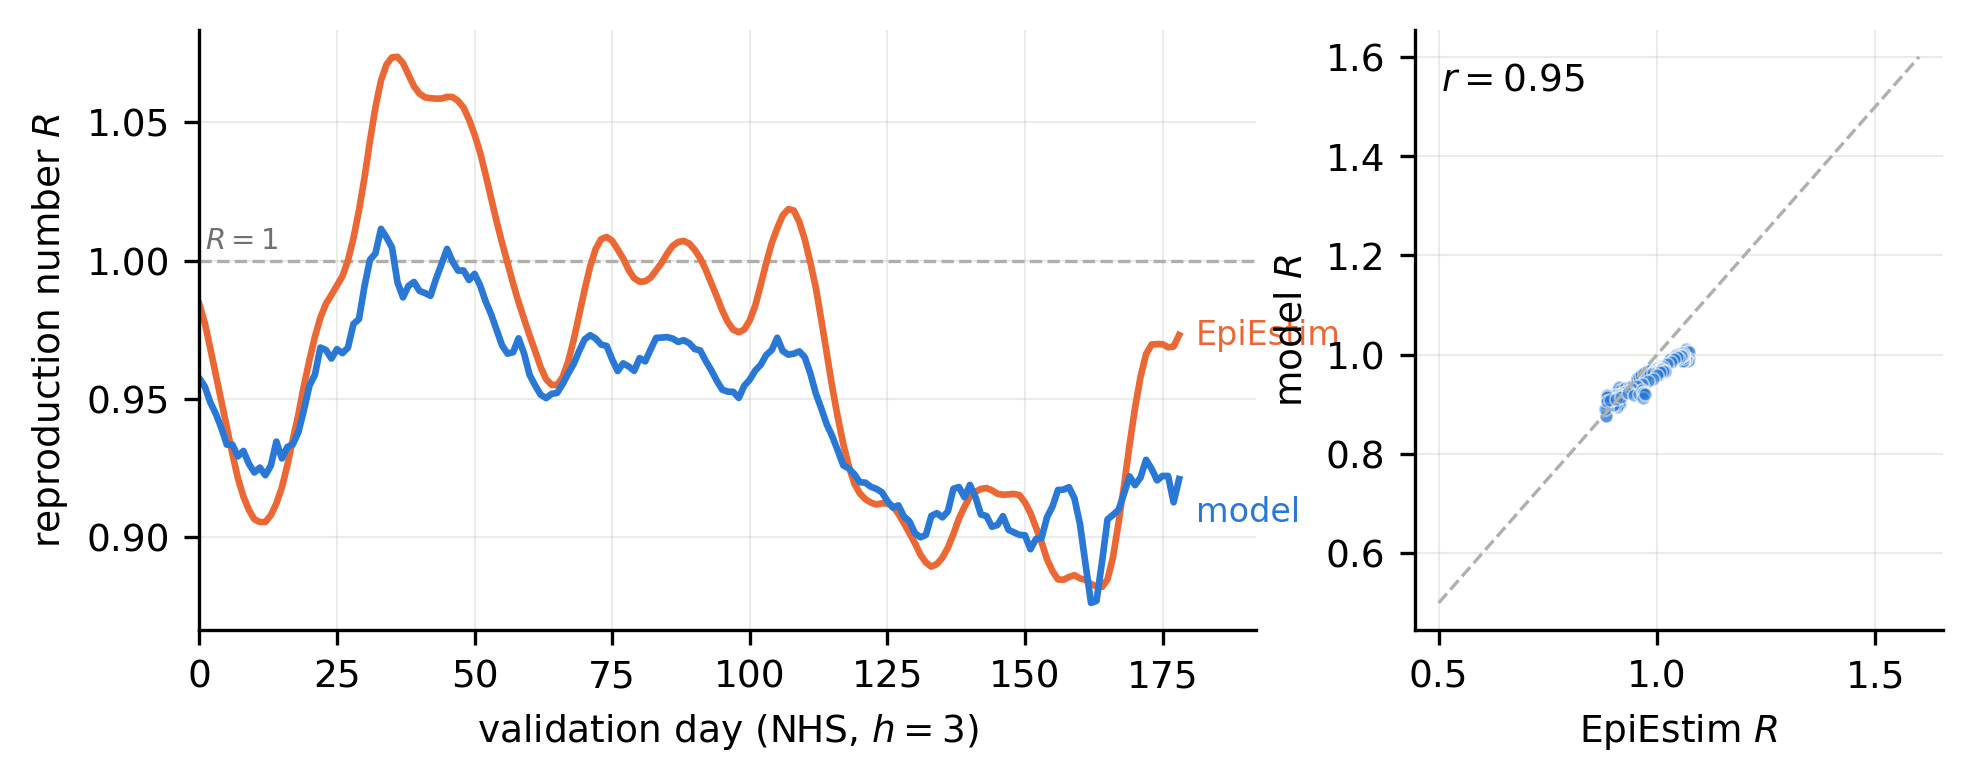
\includegraphics[width=\linewidth]{F3_r_validation}
\caption{Implied $R$ and EpiEstim (NHS, $h=3$, validation split). Left: both
series over time, with the $R=1$ threshold. Right: day-by-day scatter with
the identity line.}
\label{fig:rt}
\end{figure}

\subsection{Held-out test evaluation}
\label{sec:test}

Model development and selection used the validation split only. The test
split was evaluated once, after the configurations were frozen.

\begin{table}[ht]
\centering
\caption{Test RMSE of the four arms (NHS, mean $\pm$ SD over five seeds; bold
marks the lowest mean). The direct decoder is the identical backbone without
the renewal layer.}
\begin{tabular}{lcccc}
\hline
Horizon & Direct decoder & Learned & Uniform & Fixed (lit.) \\
\hline
$h=3$ & $2.79 \pm 0.78$ & $\mathbf{2.23 \pm 0.07}$ & $2.74 \pm 0.75$ & $3.00 \pm 1.30$ \\
$h=7$ & $7.21 \pm 2.25$ & $\mathbf{6.45 \pm 0.53}$ & $7.84 \pm 1.51$ & $7.42 \pm 1.94$ \\
$h=14$ & $13.51 \pm 5.08$ & $14.56 \pm 2.58$ & $13.53 \pm 3.79$ & $\mathbf{12.29 \pm 1.23}$ \\
\hline
\end{tabular}

\label{tab:arms-test}
\end{table}

On the test split (Table~\ref{tab:arms-test}, Fig~\ref{fig:armstest}) the
learned renewal arm has the lowest mean error at $h=3$ ($-19.9\%$ relative to
the direct decoder) and $h=7$ ($-10.6\%$), and a higher mean at $h=14$
($+7.8\%$). None of these differences is significant with five seeds: the
paired Wilcoxon test gives $p\geq0.062$, its smallest attainable value at
$n=5$, and per-timestep Diebold--Mariano tests on the median-error seeds give
$p=0.27$, $0.42$ and $0.056$, the last favouring the direct decoder. The
clearest effect concerns variance rather than the mean. The direct decoder's
test error varies widely across seeds ($2.79\pm0.78$ at $h=3$), whereas the
renewal arm is far more stable ($2.23\pm0.07$). The renewal constraint acts
as a regulariser: on this evidence it purchases stability rather than mean
accuracy.

\begin{figure}[ht]
\centering
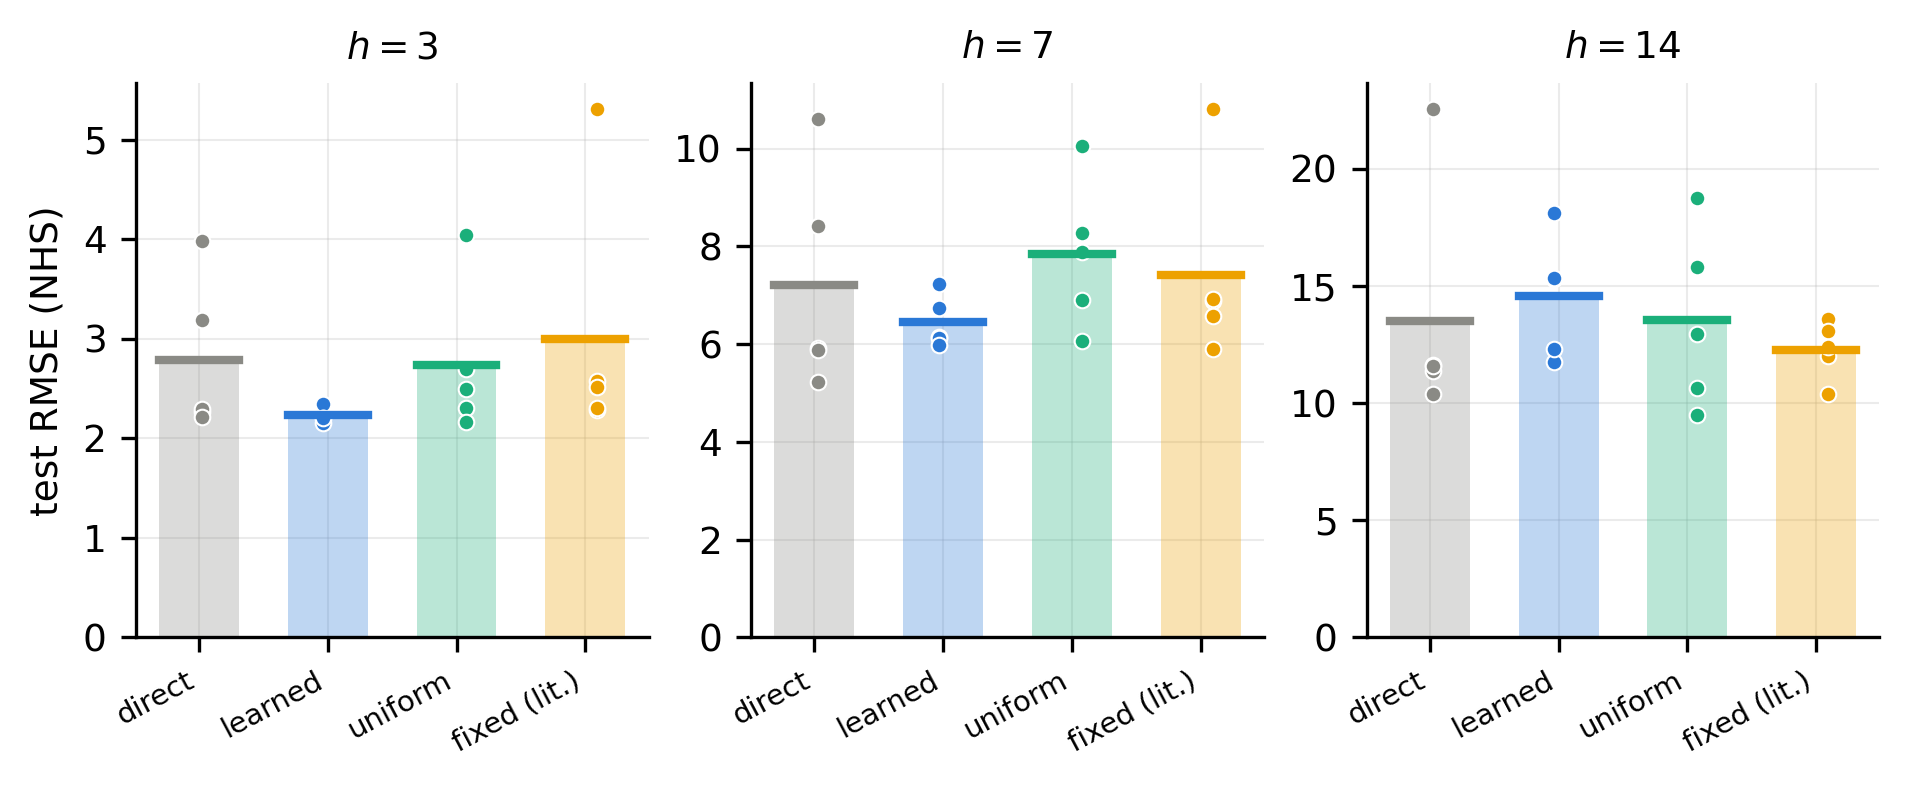
\includegraphics[width=\linewidth]{F4_arms_test}
\caption{Test RMSE by arm and horizon (NHS). Dots are individual seeds;
horizontal lines mark seed means. Note the seed spread of the direct decoder
relative to the learned renewal arm.}
\label{fig:armstest}
\end{figure}

\subsection{Search record on the selection split}
\label{sec:sweep}

For completeness, Table~\ref{tab:sweep} reports every renewal configuration
evaluated during development. All comparisons were made on the validation
split with a single seed, over five proxy cells spanning the NHS and Japanese
data. Configurations comprise single-convolution variants with kernel spans
of 7--21 steps, with and without a zero-delay term, the iterated formulation,
and residual variants with a free weight $\gamma$ on the renewal term.

None of the nine configurations won any of the forty-five cell comparisons
against the direct decoder, and the ordering is systematic: penalties shrink
as the renewal structure is weakened, and the iterated formulation, the only
one under which $\alpha_\tau$ is strictly a generation interval, does worse
than the approximate single-convolution one because iteration compounds
prediction error over $h$ feedback steps. The favourable test-split means of
Sec.~\ref{sec:test} were not visible at selection time. We conclude that
single-seed validation comparisons are unreliable in this regime, and we
report the discrepancy rather than reconciling it after the fact.

\begin{table}[ht]
\centering
\caption{Development search record (validation split, seed 42, five proxy
cells, compared against the direct decoder). Nine configurations were
evaluated; two additional runs were invalidated by a harness fault and
repeated. The count is reported for multiple-comparison transparency.}
\begin{tabular}{lcc}
\hline
Variant & Cells won (of 5) & Mean $\Delta$RMSE vs direct \\
\hline
Single conv., lag 14, $\tau{\geq}0$ & 0 & +12.5\% \\
Single conv.\ + residual $\gamma$, lag 7, $\tau{\geq}0$ & 0 & +13.4\% \\
Single conv., lag 7, $\tau{\geq}1$ & 0 & +14.3\% \\
Single conv.\ + residual $\gamma$, lag 7, $\tau{\geq}1$ & 0 & +15.9\% \\
Single conv., lag 14, $\tau{\geq}1$ & 0 & +23.4\% \\
Single conv., lag 21, $\tau{\geq}1$ & 0 & +35.0\% \\
Iterated + residual $\gamma$, lag 7 & 0 & +20.6\% \\
Iterated, lag 7 & 0 & +22.4\% \\
Iterated, lag 14 & 0 & +25.6\% \\
\hline
\end{tabular}

\label{tab:sweep}
\end{table}

\subsection{Dependence on forecast horizon}
\label{sec:threshold}

Four observations in this project show the same pattern. They are not
independent, since all share a backbone, data and splits, but they arise
from different mechanisms
(Fig~\ref{fig:threshold}). Repairing the backbone's spatial attention
(companion work) raises daily-data test error at $h=3$ ($+12.6\%$) and lowers
it at $h=7$ and $h=14$ ($-2.6\%$, $-6.1\%$). When the renewal term carries a
free weight $\gamma$, training drives $\gamma$ toward zero at $h=3$ under a
non-iterated kernel, which at that horizon reaches only observations older
than the forecast gap, while retaining $\gamma\approx0.65$--$0.70$ at
$h=7$--$14$; under the iterated kernel, $\gamma$ at $h=3$ recovers to 0.20,
and to approximately 1 on the weekly data. Kernel-shape ablations follow the
same pattern, mattering at $h\geq7$ and little at $h=3$
(Tables~\ref{tab:arms-val}, \ref{tab:arms-test}). Below a horizon of roughly
one generation interval, recent local counts dominate and structural
assumptions add noise; beyond it they contribute. Uniform improvements from
added mechanism should not be expected across horizons.

\begin{figure}[ht]
\centering
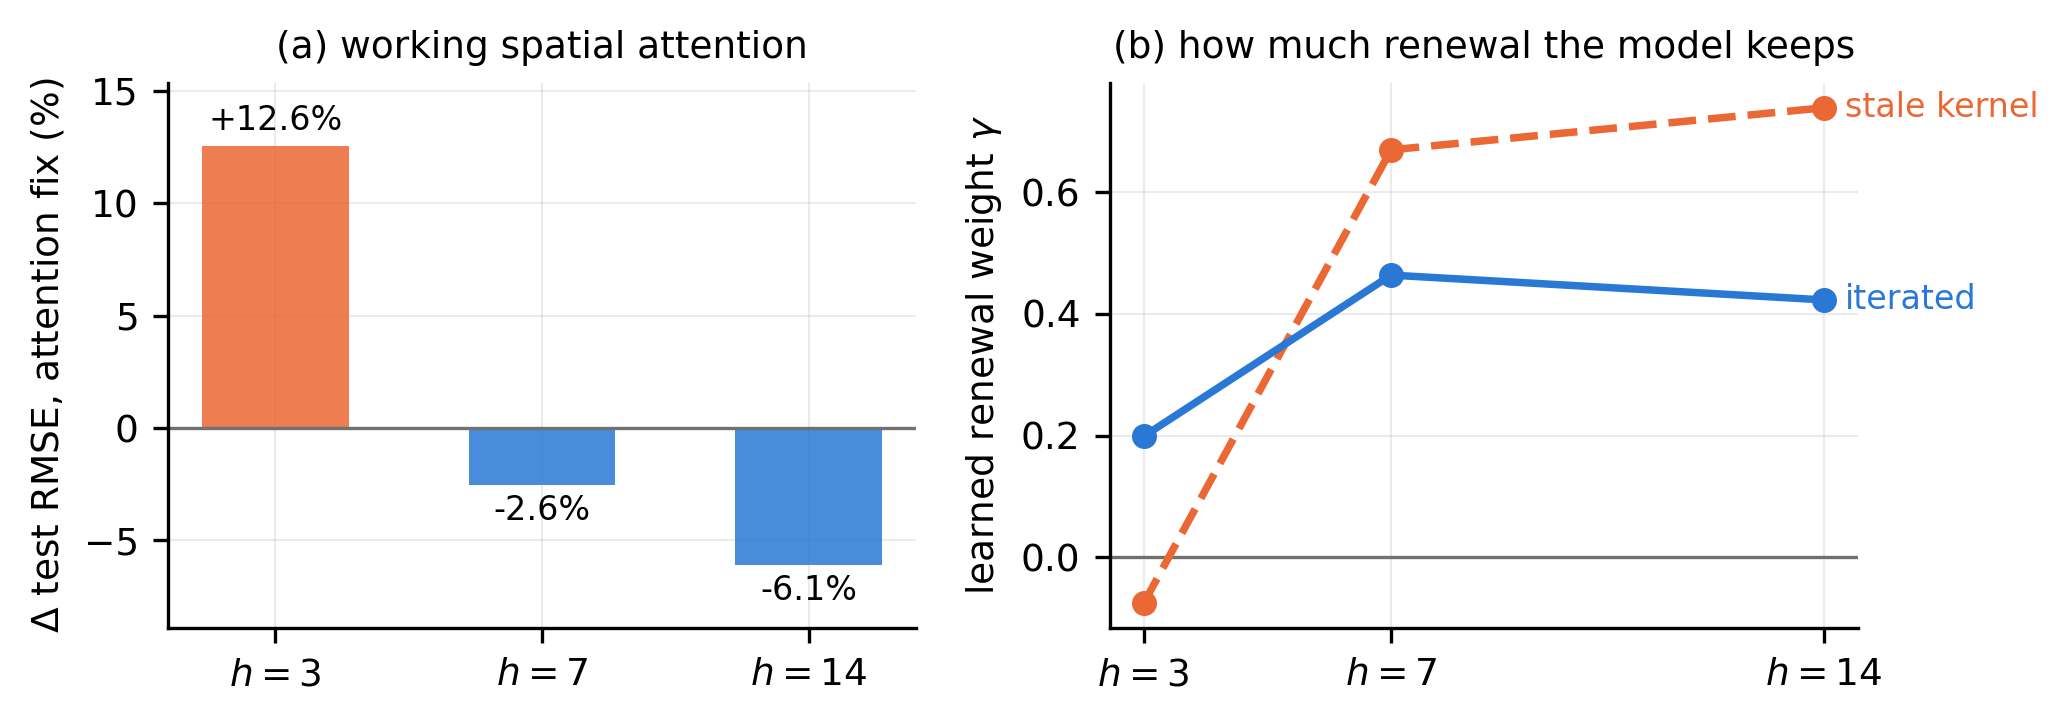
\includegraphics[width=0.95\linewidth]{F5_horizon_threshold}
\caption{Horizon dependence from two separate mechanisms. (a) Change in test
RMSE from repairing spatial attention, daily datasets. (b) The learned
renewal weight $\gamma$ (NHS) under the stale (non-iterated) kernel and the
iterated kernel.}
\label{fig:threshold}
\end{figure}

\section{Discussion}
\label{sec:discussion}

\paragraph{Mechanistic fidelity and accuracy are separate properties.} The
renewal layer recovers a generation interval consistent with contact-tracing
estimates and an \Rt consistent with EpiEstim, yet it never outperformed the
unconstrained decoder on the split used for model selection. These findings
answer different questions. A model can be mechanistically faithful where the
mechanism is identifiable from data, and mechanism need not improve point
accuracy where a flexible approximator already suffices. The same pattern has
been reported for Hawkes-process COVID-19 forecasting, where predictive skill
was attributed to the mobility-driven reproduction number rather than to the
choice of inter-infection distribution~\cite{chiang2022hawkes}, and it echoes a
broader concern that internal quantities such as attention weights do not
straightforwardly constitute explanations~\cite{jamieson2018attention}. Claims that a neural
forecaster ``learns transmission dynamics'' can be substantiated in the way
attempted here, by exposing a mechanistic quantity and comparing it with the
classical estimator, rather than by assigning epidemiological names to
internal tensors.

\paragraph{What shapes the learned kernel.} Inspection of the kernels
(Fig~\ref{fig:kernels}) shows a feature that summary statistics conceal. At
$h=3$ the kernel concentrates at $\tau=3$, which is the delay at which the
iterated decoder's convolution reaches the last observed value rather than
its own fed-back predictions; the $h=7$ kernel shows a corresponding
secondary mode at $\tau=7$. The learned kernel therefore reflects both
transmission delay and a preference for observed over self-predicted inputs.
The aggregate delay statistics fall in the plausible range regardless, but
the fine structure of the kernel should not be read as purely biological.
Separating the two influences, for instance with scheduled sampling or
supervision of intermediate steps, is a natural continuation of this work.

\paragraph{Renewal structure as regularisation.} The most consistent
test-split effect is the reduction in seed variance at short horizons, by
roughly a factor of ten. The mechanistic constraint narrows the hypothesis
space in a way that initialisation variance cannot undo. For deployment,
where a forecast consumer cannot average over seeds, an estimator with test
error $2.23\pm0.07$ may be preferable to one with $2.79\pm0.78$ even without
a significant difference in means.

\paragraph{Relation to prior work.} Classical renewal estimators fix the
generation interval~\cite{cori2013new,fraser2007estimating,
abbott2020estimating}, as do semi-mechanistic Bayesian
models~\cite{flaxman2020estimating} and the concurrent differentiable
inference method of~\cite{cirl2026conditional}, which lists learning it as
future work. Joint Bayesian estimation of reproduction number and serial
interval exists for outbreak data, but not within a spatiotemporal neural
forecaster. The delay-aware attention
literature~\cite{jiang2023pdformer,press2022train} learns delays without
epidemiological semantics. We are not aware of prior work combining these
elements: a learned kernel inside a spatially coupled neural forecaster,
trained from case counts and subsequently checked against classical
estimates.

\paragraph{Limitations.} (1) The arms study is restricted to the NHS daily
series; weekly surveillance cannot represent a sub-week generation interval,
so the Japanese analyses support conclusions about dynamics only. (2) Five
seeds bound the attainable significance level; the test-split accuracy
differences are indicative, not confirmed. (3) The iterated decoder clamps
$\log R$ to $\pm1.5$ ($R\in[0.22,4.48]$) to prevent divergence under
compounding, a constraint the direct decoder does not require. (4) The
EpiEstim comparator is a flat-prior posterior mean over a 7-day window, not a
full Bayesian posterior; the per-region analysis mitigates but does not
remove this simplification. (5) Effect sizes shrank between single-seed
exploration and multi-seed confirmation (learned versus uniform at $h=7$:
$-20\%$ on one seed, $-7\%$ over five), so single-seed comparisons in this
regime should be treated as unreliable. (6) The kernel-shape confound
described above. (7) All results are conditional on the corrected evaluation
protocol described in Methods; numbers obtained under pooled-lead protocols
are not comparable.

\section{Materials and methods}
\label{sec:methods}

\paragraph{Data.} The primary series is daily COVID-19 hospital admissions
for the seven English NHS regions, published by NHS England as part of the
COVID-19 Hospital Activity collection [TODO: insert exact URL, release and
access date]. The series comprises 895 consecutive days [TODO: confirm the
calendar range; the file begins at the first day with non-zero admissions and
runs for 895 days], covering multiple variant waves. A trailing seven-day mean
is applied at source. The secondary series is weekly influenza-like illness
counts for 47 Japanese prefectures, used only in the \Rt-dynamics analysis of
Sec.~\ref{sec:rt}. Neither series contains missing values after the leading
zeros; no imputation is performed.

Splits are chronological, 60/20/20 by time index: with 895 days this places
the train/validation boundary at day 537 and the validation/test boundary at
day 716. Min--max normalisation is fitted on the training range only. A
preprocessing audit accompanying the code verifies that no input contains
future information, that identical files are supplied to every model, and that
rolling-origin input windows may span a split boundary while targets never
precede the split start.

\paragraph{Admissions as a proxy for infections.} The renewal equation
describes infections, whereas we observe hospital admissions. Writing
admissions as a convolution of infections with a reporting delay,
$A = I \ast p$, and assuming $R$ varies slowly relative to that delay, gives
$A(t)\approx R(t)\sum_\tau w_\tau A(t-\tau)$: the renewal form is approximately
preserved for the observable with the same kernel. This approximation is why
EpiEstim is routinely applied to case, admission and death series, and both our
model and the EpiEstim comparator rely on it equally, so the comparison in
Sec.~\ref{sec:rt} is internally consistent. It is nonetheless an approximation
with known failure modes~\cite{gostic2020practical}: when $R$ changes quickly,
or when the reporting delay itself varies, the recovered kernel absorbs part of
the infection-to-admission delay structure. The kernel we report should
therefore be read as a generation interval only under this approximation, and
any residual delay structure is confounded into it. This is a second
contribution to the kernel-shape confound discussed in Sec.~\ref{sec:discussion}.

\paragraph{Spatial coupling.} Region centroids are taken from Office for
National Statistics boundary files, and the geographic prior is a symmetric
binary adjacency in which two regions are connected when their centroids lie
within 150\,km, computed by the haversine formula. For the seven NHS regions
this yields a sparse graph; the same construction at thresholds of 100, 200 and
250\,km is available in the repository. The prior enters the model only through
the row-standardised term described below and is not otherwise tuned.

\paragraph{Backbone and target space.} The backbone is a compact
spatiotemporal graph network (temporal depthwise convolutions; graph
attention over a learned low-rank bias plus a distance prior; approximately
15{,}000 parameters) trained in log-growth target space,
$g=\log\big((y_{t}+1)/(y_{t-h}+1)\big)$, with 23 quantile heads and pinball
loss. The backbone, optimiser and all hyperparameters are identical across
every arm of every comparison; only the decoder differs.

\paragraph{Renewal decoder.} The backbone output is read as $\log R_i(t+s)$
and clamped to $\pm1.5$. Incidence is reconstructed by rolling
\begin{equation}
  \hat I_i(t+s) \;=\; R_i(t+s) \sum_{\tau=1}^{L} \alpha_\tau
  \sum_j W_{ij}\, \tilde I_j(t+s-\tau), \qquad s=1..h,
\end{equation}
where $\tilde I$ denotes observed incidence for indices $\leq t$ and the
model's own predictions thereafter, $L=7$, and
$\alpha=\mathrm{softmax}(\theta)$. Because $\alpha$ is non-negative and sums
to one, the convolution commutes with the affine min--max normalisation, so
$\alpha$ retains its interpretation on the raw incidence scale. $W$ is a
row-stochastic coupling formed from a row-standardised geographic prior plus
a learned low-rank term; row-standardisation is required because softmax
attention is invariant to row-constant shifts, and row-normalising a dense
graph leaves within-row variation of order $10^{-3}$, which suppresses the
geographic signal on large graphs. The kernel begins at $\tau=1$, following
the convention $w_0=0$ of~\cite{cori2013new}; an ablation restoring $\tau=0$
appears in the search record. The layer is differentiable throughout, so
$\theta$, $W$ and the backbone parameters are trained jointly by gradient
descent on the forecast loss.

\paragraph{Training.} All models are trained with Adam (learning rate
$10^{-3}$, weight decay $5\times10^{-4}$, batch size 32) for at most 1500
epochs with early stopping on validation loss after 100 epochs without
improvement; the checkpoint with the lowest validation loss is retained. The
input window is 20 steps, hidden dimension 32, four attention heads, low-rank
bias dimension 8, dropout 0.2, and four spatial scales. Implementation is
PyTorch 2.7 on Python 3.11, trained on a single NVIDIA RTX 5060 Ti; a training
run for the seven-region series takes two to three minutes.

\paragraph{Arms.} Learned: $\theta$ free. Uniform: $\theta$ frozen at
equality. Fixed: $\theta$ frozen to the discretised gamma with mean 5.2 and
SD 1.72 days~\cite{ferretti2020quantifying}. Identical backbones and
training; seeds 42, 30, 45, 123, 1000.

\paragraph{EpiEstim comparator.} Posterior-mean Cori estimator under a flat
prior, $R_t=\sum_{s\in\mathcal{W}} I_s / \sum_{s\in\mathcal{W}} \Lambda_s$
with $\Lambda_s=\sum_\tau w_\tau I_{s-\tau}$, a trailing 7-day window
$\mathcal{W}$, and the literature $w$. The model's implied $R$ is the
per-step $\exp(\log R)$ averaged over the horizon for the aggregate analysis,
or taken per node for the per-region analysis.

\paragraph{Statistics.} Multi-seed cells report mean $\pm$ SD
(\textsc{ddof}=1). Paired comparisons across seeds use the exact Wilcoxon
signed-rank test. Per-timestep comparisons use Diebold--Mariano with
Newey--West long-run variance at lag $h-1$, the Harvey--Leybourne--Newbold
small-sample correction, and $t_{n-1}$ critical values; where families of
comparisons are reported elsewhere in the project, Holm correction is applied
within families. Interval forecasts elsewhere in the project are scored with
the weighted interval score~\cite{bracher2021evaluating}.

\paragraph{Evaluation protocol.} All models are scored at lead $h$ exactly.
We state this explicitly because an audit of our own earlier work found
baseline models scored on pooled leads $h..2h{-}1$ against a lead-$h$
proposal, an asymmetry that inflated apparent margins; every model was
retrained under the single-lead protocol, and the audit is reported in a
companion paper.

\paragraph{Reproducibility.} All tables are generated by script from
persisted result files and checkpoints (\texttt{paper\_tables.py}), and all
figures likewise (\texttt{paper\_figures.py}). The development search
record, including invalidated runs, is preserved in the repository ledger.

\section*{Acknowledgements}
[To be completed.]

\section*{Financial disclosure}
[To be completed. If no specific funding applies: ``The authors received no
specific funding for this work.'']

\section*{Competing interests}
The authors have declared that no competing interests exist.

\section*{Author contributions}
[To be completed after co-author confirmation.]

\section*{Data and code availability}
Code, configuration ledgers and prediction artefacts are available in the
project repository; the NHS and Japanese surveillance datasets are public.
[Repository URL to be added.]

\bibliographystyle{unsrtnat} % swap for plos2015.bst at submission
\bibliography{renewal}

\end{document}
